
\section{Current architecture}

\begin{frame}{Current SeismoCloud architecture}
\centering
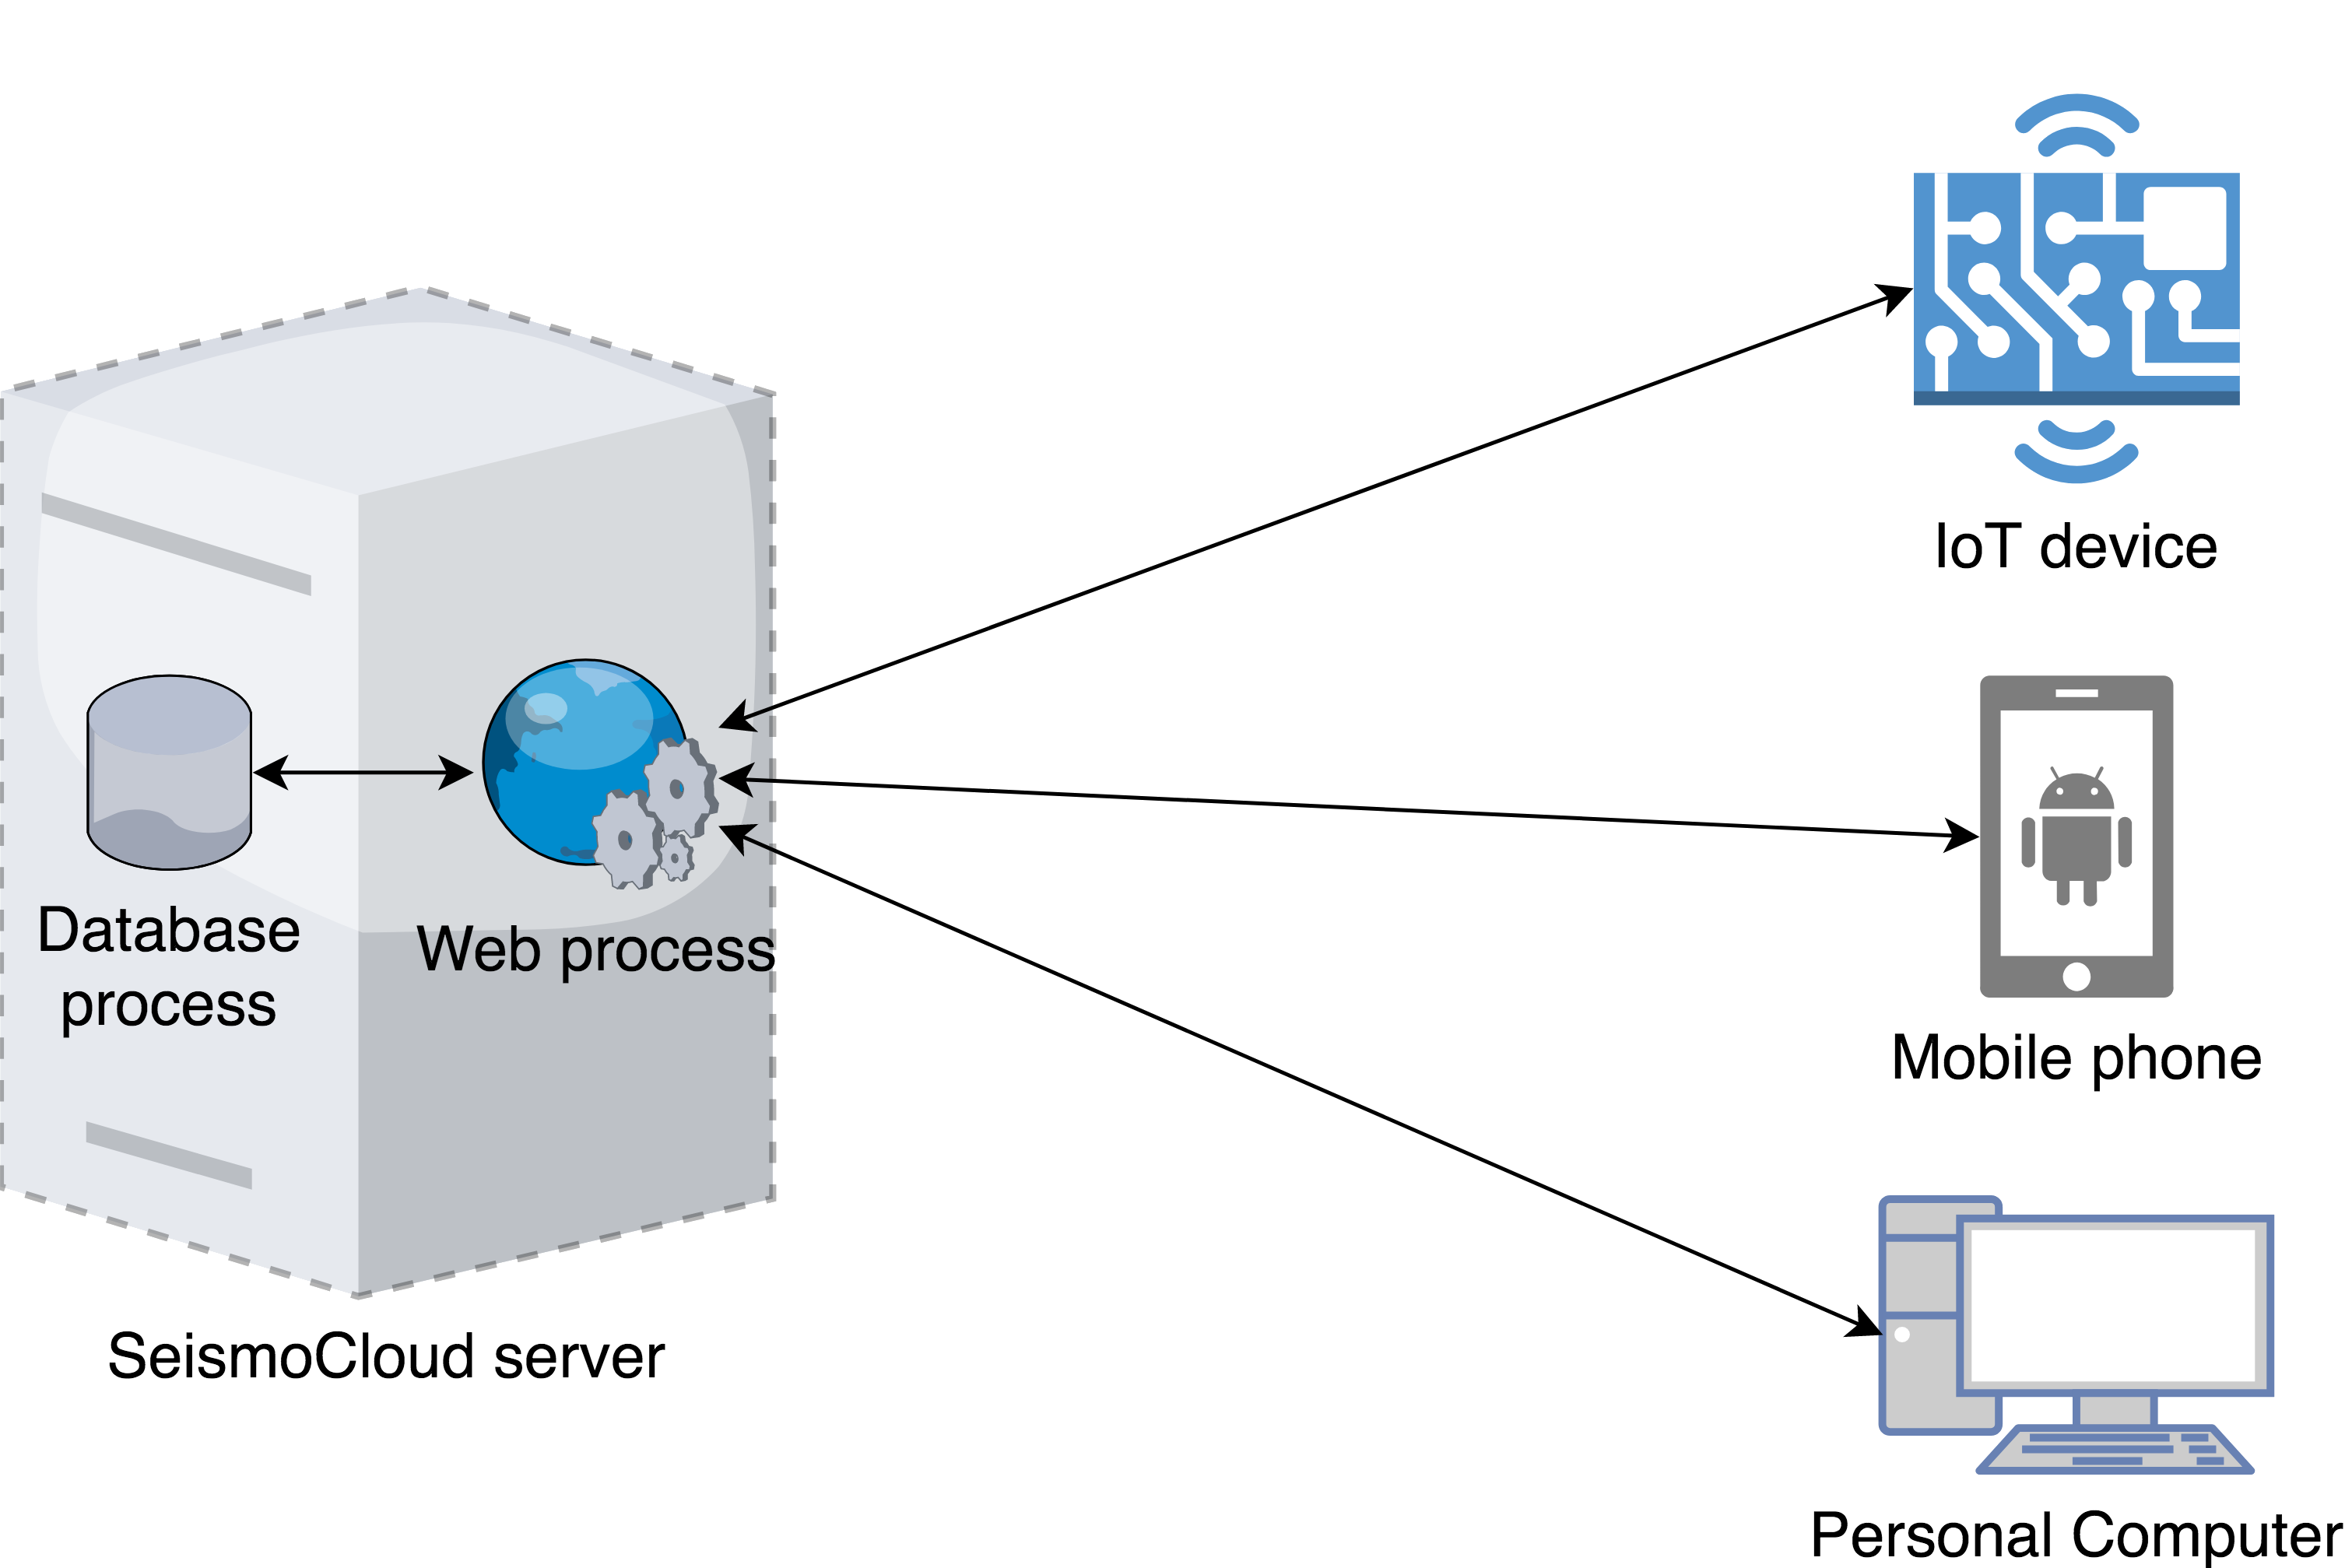
\includegraphics[width=0.8\textwidth]{scs-current-architecture}
\end{frame}


\begin{frame}{Current SeismoCloud architecture: numbers}
\begin{itemize}
  \item \textbf{Users}: \circa 13k devices, nearly 10k users
  \item \textbf{Wide area}: wide adoption in the EU, Mexico, west coast of US
  and south America
  \item \textbf{Computing power}: 2 x 2.4 GHz Intel CPU, avg load \circa 60\%
  \item \textbf{Memory}: 5 GB of RAM, avg load \circa 80\%
  \item \textbf{Storage}: +20 GB (both current and historical data)
  \item \textbf{Cost}: \circa 1400 € per year (server maintenance is made by us)
\end{itemize}

\textbf{Data collected in a quiet situation - eg. no major earthquakes}
\end{frame}


\begin{frame}{Current SeismoCloud architecture: map}
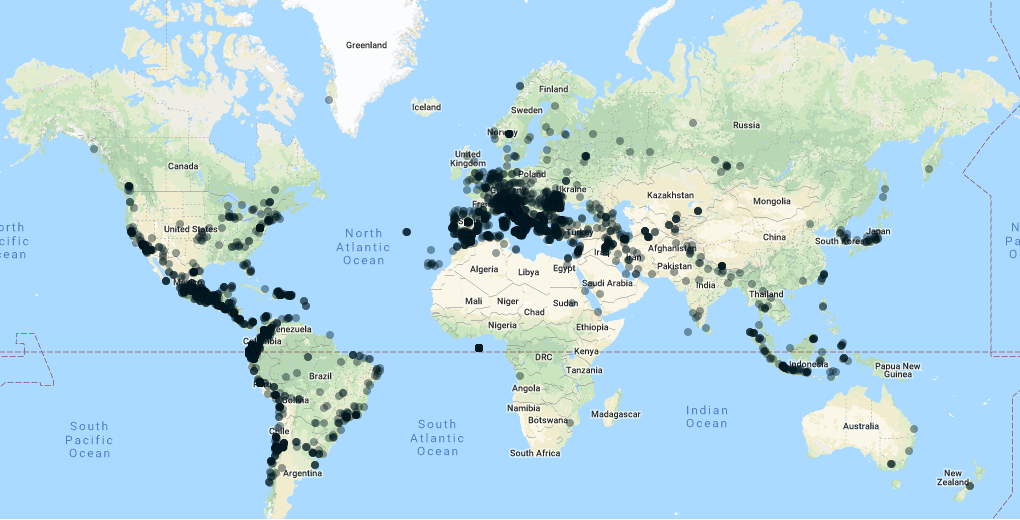
\includegraphics[width=\textwidth]{seismocloud_network}
\end{frame}


\begin{frame}{Current SeismoCloud architecture: issues}
\begin{itemize}
  \item \textbf{Limited scalability}: only vertical scalability. There is no way
  to scale the system horizontally due design flaws
  \item \textbf{No elasticity}: the system cannot adapt automatically to match
  workload changes over time
  \item \textbf{No high availability}: only one server manages (nearly) all. If
  it's down, the project is gone
  \item \textbf{Under provisioning}: the system is highly under-provisioned:
  necessary resources to handle a big network activity (such as a big earthquake)
  are missing
  \item \textbf{Over provisioning}: the system is over-provisioned for quiet
  periods of time (eg. no earthquakes)
\end{itemize}
\end{frame}


\begin{frame}{Current SeismoCloud architecture: improvements}
	A recent study highlighted the fact that HTTP(s) is not the right protocol to
	run a system like SeismoCloud, due many technical facts. The same study suggests
	to implement a \textit{Message-based, Publish-Subscription} protocol like
	\textbf{MQTT}, Message Queue Transport Protocol.

	\vspace{1em}

	The MQTT protocol needs a specialized software, named \textit{MQTT Broker}.
	The \textit{MQTT Broker} software needs to run in a server, and it will become
	vital for the project.

	\vspace{1em}

	Also, a gateway between MQTT and HTTP needs to be written from scratch: we named
	it \textit{SeismoCloud controller}. Even the \textit{SeismoCloud controller}
	will be part of the vital components.

\end{frame}
